\subsubsection{UC14 - Gestione acquisti e vendite}
\begin{figure}[h]
	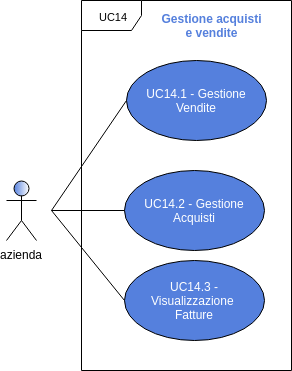
\includegraphics[width=6cm]{res/images/UC14-Generale.png}
	\centering
	\caption{Gestione degli acquisti e delle vendite da parte delle aziende}
\end{figure}
\begin{itemize}
	\item \textbf{Attori Primari}: azienda;
	\item \textbf{Descrizione}: alle aziende sono messe a disposizione diverse operazione per visualizzare e gestire le vendite e gli acquisti che vengono effettuati all'interno della piattaforma. Inoltre è possibile visualizzare lo storico di tutte le fatture;
	\item \textbf{Scenario principale}: l'utente visualizza e svolge alcune operazioni per gestire le vendite, gli acquisti e le fatture ad essi riguardanti;
	\item \textbf{Precondizione}: il sistema ha riconosciuto l'utente autenticato come azienda, e mette a disposizione tutte le pagine necessarie alla visualizzazione e gestione degli acquisti, vendite e fatture.
	\item \textbf{Postcondizione}: l'azienda ha visualizzato e/o gestito i propri acquisti, vendite e fatture.
\end{itemize} 
\subsubsection{UC14.1 - Gestione vendite}
\begin{figure}[H]
	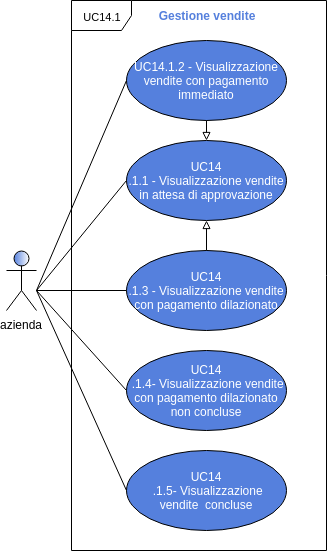
\includegraphics[width=8cm]{res/images/UC14-Vendite.png}
	\centering
	\caption{Gestione delle vendite da parte delle aziende}
\end{figure}
\begin{itemize}
	\item \textbf{Attori Primari}: azienda;
	\item \textbf{Descrizione}: alle aziende sono messe a disposizione diverse operazione per visualizzare e gestire le vendite all'interno della piattaforma. Esse comprendono la visualizzazione dello stato di approvazione/rifiuto di proposte d'ordine verso altre aziende, l'approvazione/rifiuto di proposte di pagamento dilazionato, e la visualizzazione delle aziende che devono ancora pagare una somma dilazionata come precedentemente accordato;
	\item \textbf{Scenario principale}: l'utente visualizza e svolge alcune operazioni per gestire le vendite;
	\item \textbf{Precondizione}: il sistema ha riconosciuto l'utente autenticato come azienda, e mette a disposizione tutte le pagine necessarie alla visualizzazione e gestione delle vendite;
	\item \textbf{Postcondizione}: l'azienda ha visualizzato e/o gestitole proprie vendite.
\end{itemize} 

\subsubsection{UC14.1.1 - Visualizzazione vendite in attesa di approvazione}
\begin{itemize}
	\item \textbf{Attori Primari}: azienda;
	\item \textbf{Descrizione}: l'azienda può visualizzare la lista delle vendite la cui proposta d'ordine deve essere ancora accettata dall'azienda cliente;
	\item \textbf{Scenario principale}: l'utente visualizza la lista delle vendite la cui proposta d'ordine deve essere ancora accettata dall'azienda cliente;
	\item \textbf{Specializzazione}:
	\begin{itemize}
		\item \textbf{UC14.1.2}: visualizzazione della precedente lista filtrando per le vendite a pagamento immediato;
		\item \textbf{UC14.1.3}: visualizzazione della precedente lista filtrando per le vendite a pagamento dilazionato\glo;
	\end{itemize}
	\item \textbf{Precondizione}: il sistema ha riconosciuto l'utente autenticato come azienda, e questo ha espresso la volontà di visualizzare la lista delle vendite la cui proposta d'ordine deve ancora essere gestita dall'azienda cliente;
	\item \textbf{Postcondizione}: l'azienda visualizza tale lista.
\end{itemize}


\subsubsection{UC14.1.2 - Visualizzazione vendite con pagamento immediato}
\begin{itemize}
	\item \textbf{Attori Primari}: azienda;
	\item \textbf{Descrizione}: l'azienda può visualizzare la lista delle vendite la cui proposta d'ordine deve essere ancora accettata dall'azienda cliente, mostrando esclusivamente i risultati relativi alle vendite con modalità di pagamento immediato;
	\item \textbf{Scenario principale}: l'utente visualizza la lista delle vendite la cui proposta d'ordine deve essere ancora accettata dall'azienda cliente. Vengono mostrati esclusivamente i risultati relativi alle vendite con modalità di pagamento immediato;
	\item \textbf{Precondizione}: il sistema ha riconosciuto l'utente autenticato come azienda, e questo ha espresso la volontà di visualizzare la lista delle vendite la cui proposta d'ordine deve ancora essere gestita dall'azienda cliente, visualizzando solo le vendite con modalità di pagamento immediato;
	\item \textbf{Postcondizione}: l'azienda visualizza tale lista.
\end{itemize}


\subsubsection{UC14.1.3 - Visualizzazione vendite con pagamento dilazionato}
\begin{itemize}
	\item \textbf{Attori Primari}: azienda;
	\item \textbf{Descrizione}: l'azienda può visualizzare la lista delle vendite la cui proposta d'ordine deve essere ancora accettata dall'azienda cliente, mostrando esclusivamente i risultati relativi alle vendite con modalità di pagamento dilazionato\glo;
	\item \textbf{Scenario principale}: l'utente visualizza la lista delle vendite la cui proposta d'ordine deve essere ancora accettata dall'azienda cliente. Vengono mostrati esclusivamente i risultati relativi alle vendite con modalità di pagamento dilazionato\glo;
	\item \textbf{Precondizione}: il sistema ha riconosciuto l'utente autenticato come azienda, e questo ha espresso la volontà di visualizzare la lista delle vendite la cui proposta d'ordine deve ancora essere gestita dall'azienda cliente, visualizzando solo le vendite con modalità di pagamento dilazionato\glo;
	\item \textbf{Postcondizione}: l'azienda visualizza tale lista.
\end{itemize}


\subsubsection{UC14.1.4 - Visualizzazione vendite con pagamento dilazionato non concluse}
\begin{itemize}
	\item \textbf{Attori Primari}: azienda;
	\item \textbf{Descrizione}: l'azienda può visualizzare la lista delle vendite con pagamento dilazionato\glosp non ancora concluse, ovvero l'azienda-cliente deve ancora effettuare il pagamento;
	\item \textbf{Scenario principale}: l'utente visualizza la lista delle vendite con modalità di pagamento dilazionato\glosp accettate ma non ancora concluse;
	\item \textbf{Precondizione}: il sistema ha riconosciuto l'utente autenticato come azienda, e questo ha espresso la volontà di visualizzare la lista delle vendite con modalità di pagamento dilazionato\glosp accettate ma non ancora concluse;
	\item \textbf{Postcondizione}: l'azienda visualizza tale lista.
\end{itemize}

\subsubsection{UC14.1.5 - Visualizzazione vendite concluse}
\begin{itemize}
	\item \textbf{Attori Primari}: azienda;
	\item \textbf{Descrizione}: l'azienda può visualizzare la lista delle vendite concluse;
	\item \textbf{Scenario principale}: l'utente visualizza la lista delle vendite concluse, con specificato l'avvenuto successo o meno (rifiuto della proposta d'ordine da parte dell'azienda cliente);
	\item \textbf{Precondizione}: il sistema ha riconosciuto l'utente autenticato come azienda, e questo ha espresso la volontà di visualizzare la lista delle vendite concluse;
	\item \textbf{Postcondizione}: l'azienda visualizza tale lista.
\end{itemize}

\subsubsection{UC14.2 - Gestione acquisti}
\begin{figure}[h]
	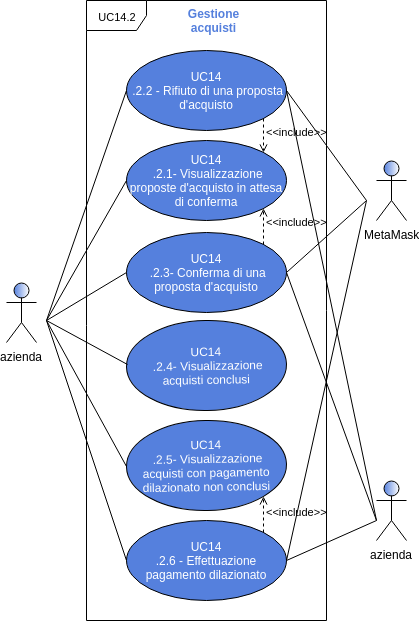
\includegraphics[width=8cm]{res/images/UC14-Acquisti.png}
	\centering
	\caption{Gestione degli acquisti da parte delle aziende}
\end{figure}
\begin{itemize}
	\item \textbf{Attori Primari}: azienda;
	\item \textbf{Descrizione}: alle aziende sono messe a disposizione diverse operazione per visualizzare e gestire gli acquisti all'interno della piattaforma. Esse comprendono la visualizzazione degli ordini in attesa di conferma, degli acquisti conclusi, e degli acquisti con pagamento dilazionato ancora da estinguere. Inoltre è possibile effettuare il pagamento di quest'ultimi;
	\item \textbf{Scenario principale}: l'utente visualizza e svolge alcune operazioni per gestire i propri acquisti;
	\item \textbf{Precondizione}: il sistema ha riconosciuto l'utente autenticato come azienda, e mette a disposizione tutte le pagine necessarie alla visualizzazione e gestione delle vendite;
	\item \textbf{Postcondizione}: l'azienda ha visualizzato e/o gestitole proprie vendite.
\end{itemize} 



\subsubsection{UC14.3 - Gestione Fatture}
\begin{itemize}
	\item \textbf{Attori Primari}: azienda;
	\item \textbf{Descrizione}: alle aziende sono messe a disposizione diverse operazione per visualizzare e gestire le fatture riguardanti gli acquisti e le vendite all'interno della piattaforma.
	\item \textbf{Scenario principale}: l'utente visualizza le fatture riguardanti gli acquisti e le vendite;
	 
	\item \textbf{Precondizione}: il sistema ha riconosciuto l'utente autenticato come azienda, l'utente ha espresso la volontà di visualizzare le fatture;
	\item \textbf{Postcondizione}: l'azienda ha visualizzato e/o gestitole proprie vendite.
\end{itemize} 
